\chapter{Realizações}\label{chp:realizacoes}

\section{Estudos em desenvolvimento Android Studio}

O desenvolvimento de aplicativos para \textit{Android} foi estudado nos primeiros meses da pesquisa. Nessa parte do projeto, a pesquisa teve um aspecto mais técnico, que foi necessário para a programação das futuras aplicações que estariam por vir. A \textit{IDE} (ambiente de desenvolvimento integrado) utilizada foi o \textit{Android Studio}, que foi sugerida pelo curso adquirido da \textit{Udemy} \cite{udemy}.

Após as primeiras semanas de aprendizado \textit{Android}, foi iniciado uma pesquisa sobre o desenvolvimento de aplicativos voltados a realidade aumentada. Porém, antes de irmos diretamente nisso, um interessante teste foi realizado com \textit{OpenCV},  que consistiu em realizar a primeira manipulação das imagens da câmera \cite{opencv}. A experiência foi proveitosa para o aprendizado da integração de ferramentas externas ao projeto padrão da plataforma e que, ademais, será feito muitas vezes até a conclusão da pesquisa.

A primeira biblioteca de realidade aumentada a ser testada foi o \textit{Google Sceneform} \cite{Sceneform}. Muitos problemas foram encontrados na integração dos \textit{plugins} com o \textit{Android Studio}, pois este precisava estar em uma versão antiga específica para funcionar. Após a instalação, foi possível ver a primeira projeção em realidade aumentada em um simulador de \textit{smartphone} no computador (figura \ref{fig:sceneform-sim}). Restava testar o aplicativo para um \textit{smartphone} real, porém o afastamento dos integrantes do laboratório pela pandemia, e a falta de dispositivos compatíveis à minha disposição, causaram um atraso nos testes. Felizmente, foi gerado um arquivo que permite a instalação à distância e o aplicativo funcionou com sucesso nos celulares da equipe (figura \ref{fig:sceneform-real}).

\begin{figure}[ht]
\centering
    \begin{subfigure}{.45\textwidth}
        \centering
        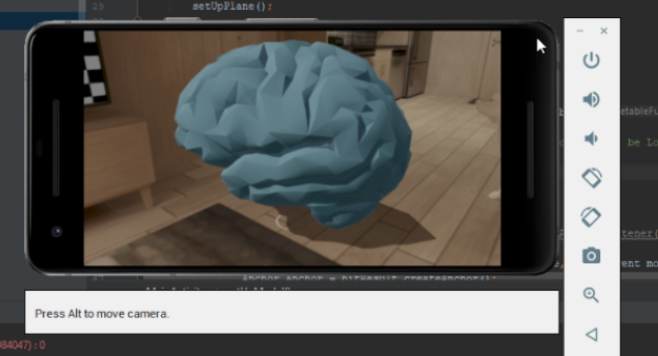
\includegraphics[width=.95\textwidth]{figuras/sceneform.png}
        \caption{Simulação da projeção AR }
        \label{fig:sceneform-sim}
    \end{subfigure}
    \begin{subfigure}{.45\textwidth}
        \centering
        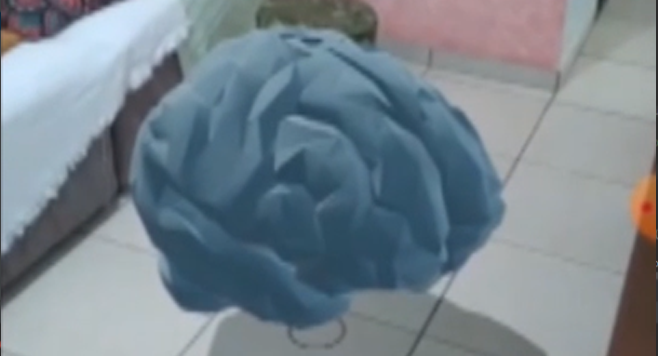
\includegraphics[width=.95\textwidth]{figuras/sceneformAR.png}
        \caption{Teste do aplicativo com \textit{Smartphone} real}
        \label{fig:sceneform-real}
    \end{subfigure}
    \caption{Resultados adquiridos com o \textit{Google Sceneform}. Fonte: Autor.}
    \label{fig:sceneform-tests}
\end{figure}

Prosseguindo os estudos de aplicativos AR, percebemos que os problemas de versão tidos com o \textit{Sceneform} estavam sendo reparados pelo \textit{Google}e adaptados em um novo programa: \textit{Google ARCore Services} \cite{arcore-googleplay}. Sua proposta é que uma biblioteca seja instalada no celular para que os aplicativos tenham acesso, trazendo a vantagem da redução do tamanho das aplicações produzidas. No entanto, somente uma lista restrita de \textit{smartphones} modernos podem instalar essa biblioteca, a justificativa dos desenvolvedores é a compatibilidade com o sistema \cite{arcore-list}.

Seguido disso, durante a pesquisa foi encontrado uma nova ideia \textit{open-source}, também do \textit{Google}, chamado \textit{Mediapipe}, que tinha a proposta de entregar muitas ferramentas de visão computacional com ML (\textit{machine learning}) integrado \cite{mediapipe-docs}. O projeto foi iniciado em julho de 2019, e tem ganhado mais popularidade por ser gratuito, multi-plataforma e facilitar muito a aplicação de ML para \textit{Android}, \textit{iOS}, e PC. No momento da descoberta, não era conhecido a compatibilidade do \textit{Mediapipe} com \textit{API} antigas de \textit{Android} e muito menos o seu comportamento em óculos de realidade aumentada, por isso, a ideia foi reservada.

\begin{description}
   \item Um sumário das opções testadas com breves comentários abaixo:
   \item[\textit{Google Sceneform}] É um \textit{plugin} para \textit{Android Studio} que introduz muitas ferramentas para o desenvolvimento de aplicativos AR. Funciona somente em \textit{Android} com a \textit{API} 24 ou superior. Seu projeto foi arquivado em meados de 2020. 
   \item[\textit{Google ARCore Services}] Pode se considerar o sucessor das ideias do \textit{Sceneform}. Ele fornece uma biblioteca de ferramentas sofisticadas para AR e atualizações frequentes. Funciona somente em uma lista estrita de \textit{smartphones} modernos. 
   \item[\textit{Mediapipe}] Fornece uma grande quantidade de ferramentas baseadas em \textit{Machine Learning} para visão computacional. Projeto iniciado em junho de 2019 e ganhando mais força recentemente. Pela recente criação, não é conhecido seu comportamento em \textit{API} antigas (28 ou anterior).
\end{description}

% \begin{figure}[ht]
% \centering
%     \begin{subfigure}{0.45\textwidth}
%         \centering
%         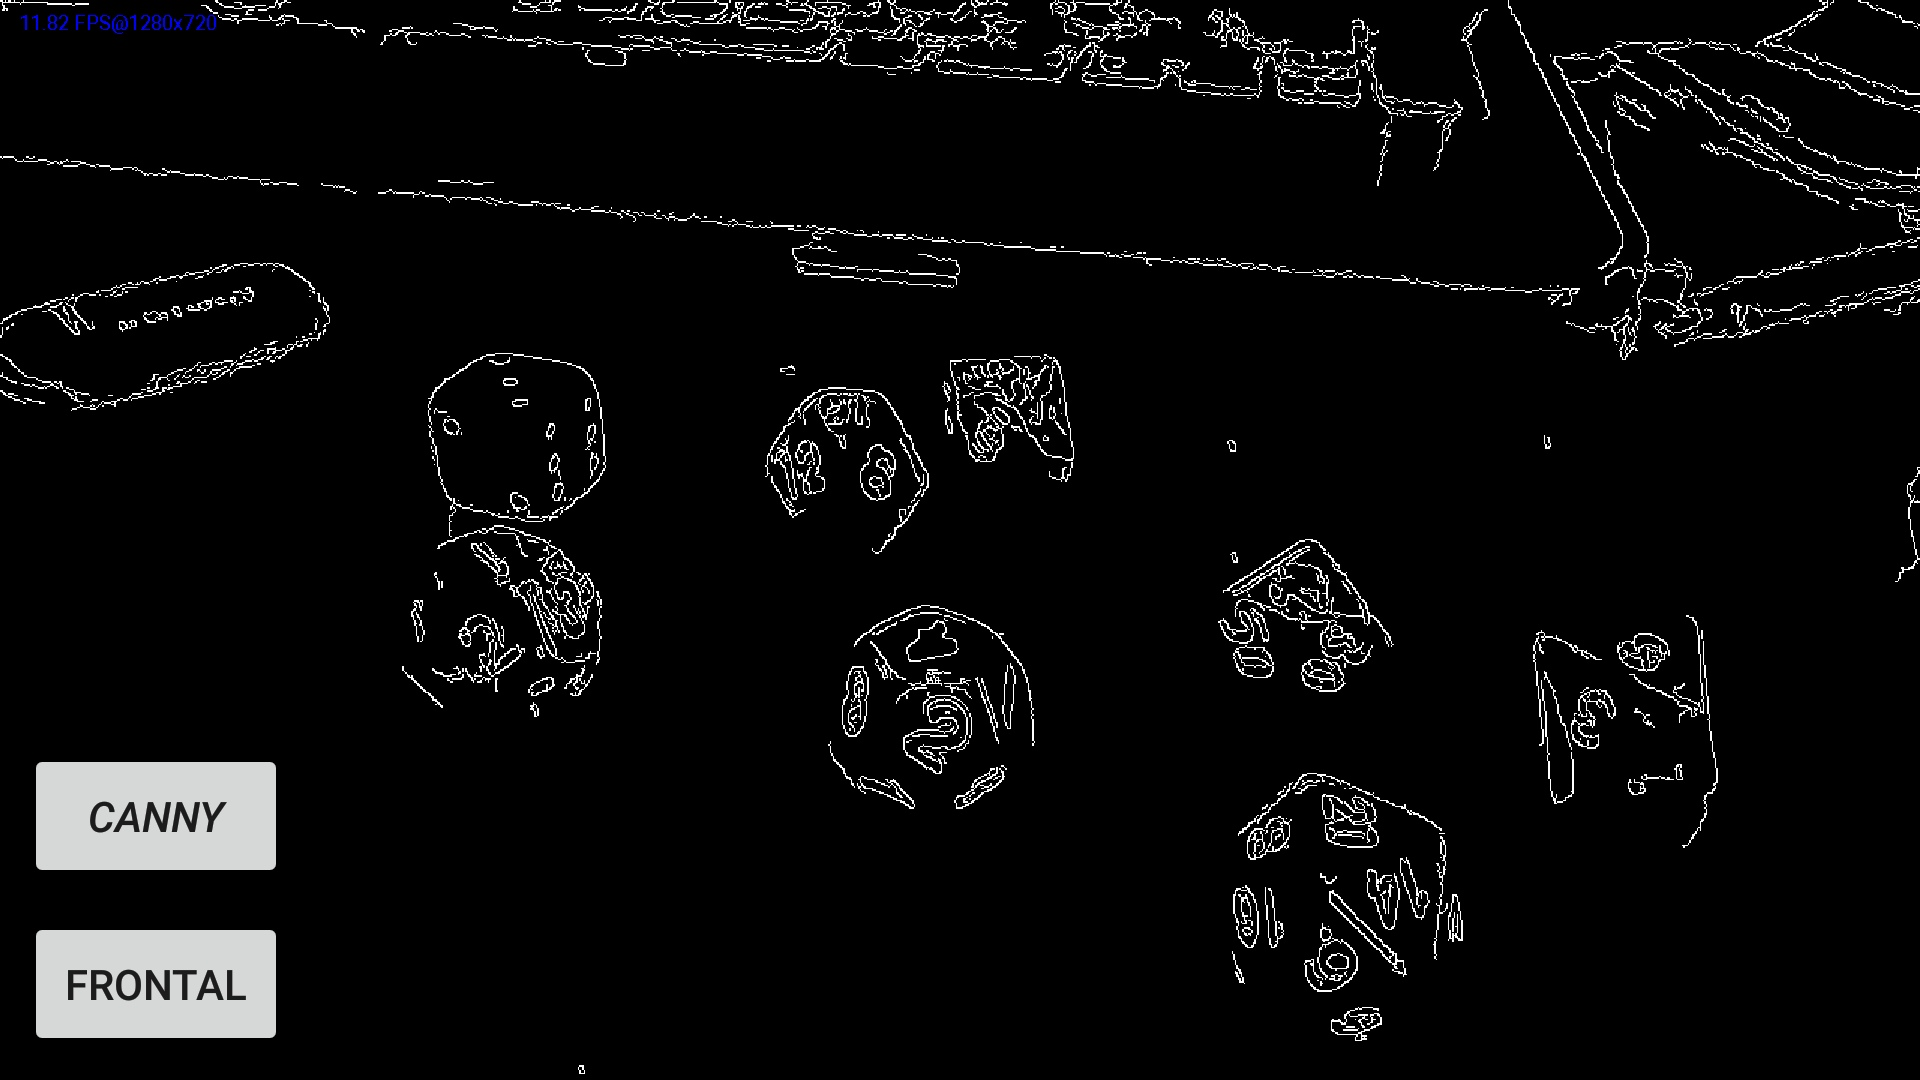
\includegraphics[width=.95\textwidth]{figuras/opencv-canny.jpg}
%         \caption{Aplicativo com \textit{OpenCV} integrado no \textit{Android}}
%         \label{fig:canny}
%     \end{subfigure}
%     \begin{subfigure}{0.45\textwidth}
%         \centering
%         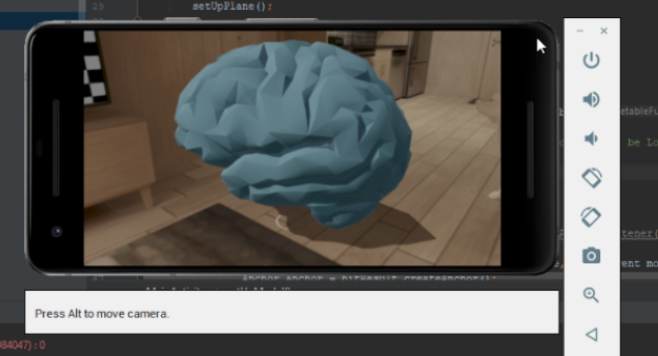
\includegraphics[width=.95\textwidth]{figuras/sceneform.png}
%         \caption{Primeiro aplicativo AR para \textit{Android}}
%         \label{fig:sceneform}
%     \end{subfigure}
%     \begin{subfigure}{0.45\textwidth}
%         \centering
%         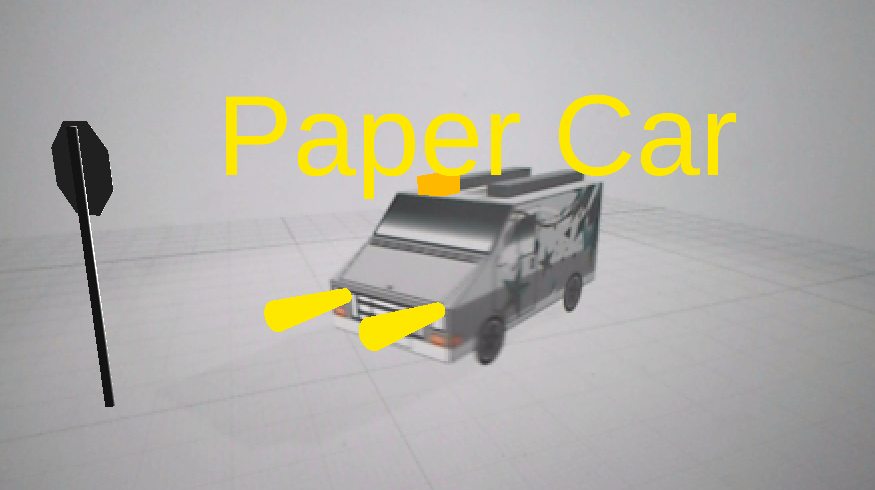
\includegraphics[width=.95\textwidth]{figuras/PaperCarAR.png}
%         \caption{Aplicativo de exemplo fornecido pela \textit{EPSON}}
%         \label{fig:papercarr}
%     \end{subfigure}
%     \begin{subfigure}{0.45\textwidth}
%         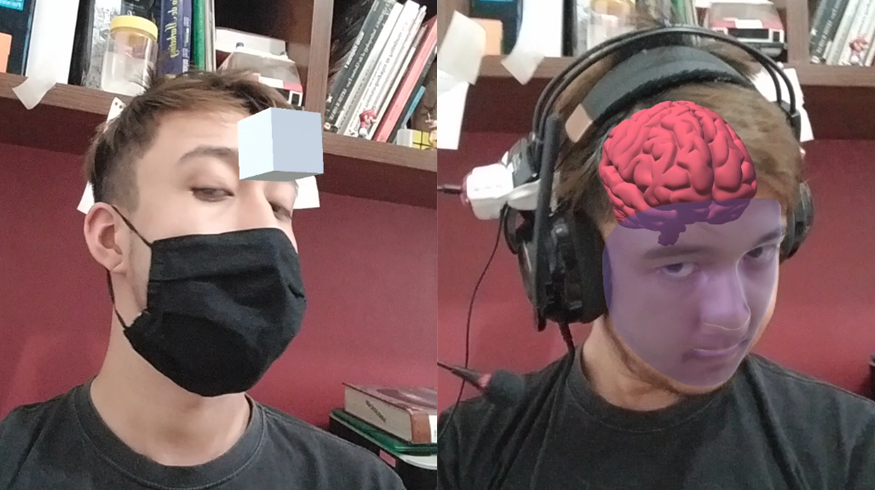
\includegraphics[width=.95\linewidth]{figuras/VCranium.png}
%         \caption{Primeira versão do \textit{VCranium}}
%         \label{fig:vcranium_alpha}
%     \end{subfigure}
%     \caption{Histórico de realizações da pesquisa até a primeira entrega parcial. Fonte: Autor.}
%     \label{fig:historico}
% \end{figure}

O que podemos concluir do desenvolvimento de aplicações em realidade aumentada com \textit{Android Studio} é que mesmo existindo ferramentas robustas de criação de \textit{apps} em AR, eles são restritos às novas versões de \textit{Android}, que por sua vez, estão presentes somente em dispositivos de nova geração, i.e, de lançamento posteriores a 2018. Por fim, a incompatibilidade das bibliotecas com o sistema e a construção dos óculos AR foram os motivos para a procura de um novo ambiente de desenvolvimento, que seja mais versátil e comporte bem com os recursos do \textit{Moverio BT-350}.

\section{Estudos de desenvolvimento Unity}

\textit{Unity} é um programa voltado para o desenvolvimento de jogos em múltiplas plataformas, sendo o \textit{Android} uma delas, e com o apoio da USP, temos acesso a mais recursos para os projetos desenvolvidos nele \cite{UnityOficial}. A documentação da \textit{EPSON} forneceu um programa de exemplo para \textit{Unity} que pode reconhecer um certo carrinho de papel e sobrepor com animações em AR.

Foi sugerido a impressão e a montagem do carrinho de papel pela documentação, porém, como os óculos possuem somente uma \textit{webcam} simples para a detecção, supomos que ele não pode diferenciar o carrinho real de uma fotografia do carrinho, então, ele funcionaria normalmente com uma imagem do computador. De fato, isso ocorreu e o teste foi registrado nas figuras \ref{fig:papercar-stl} e \ref{fig:papercar-ar}.

\begin{figure}[ht]
    \centering
        \begin{subfigure}{.45\textwidth}
            \centering
            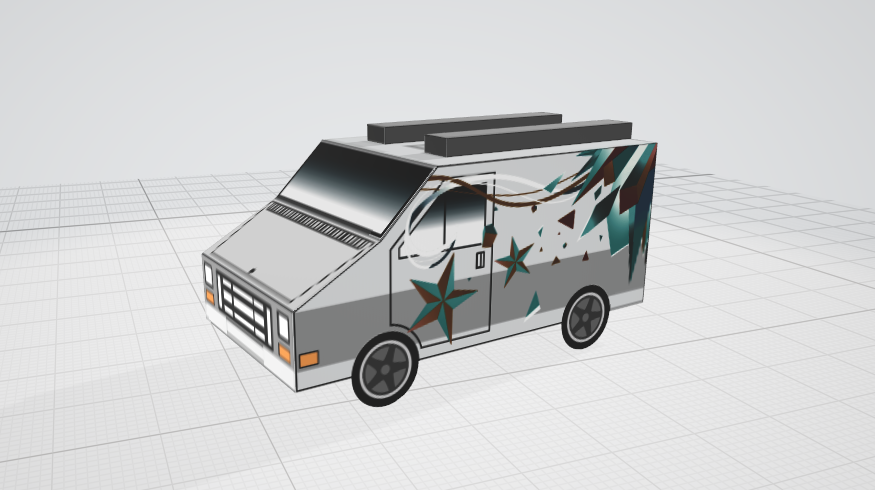
\includegraphics[width=.95\textwidth]{figuras/PaperCar.png}
            \caption{Modelo virtual do carrinho de papel}
            \label{fig:papercar-stl}
        \end{subfigure}
        \begin{subfigure}{.45\textwidth}
            \centering
            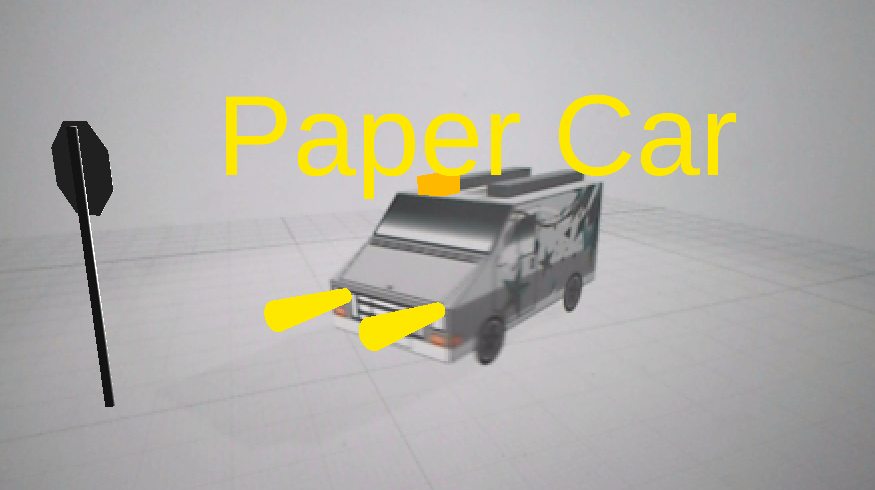
\includegraphics[width=.95\textwidth]{figuras/PaperCarAR.png}
            \caption{Sobreposição em AR com \textit{Moverio}}
            \label{fig:papercar-ar}
        \end{subfigure}
        \caption{Resultados adquiridos dos testes da documentação \textit{Moverio} no \textit{Unity}. Fonte: Autor.}
        \label{fig:papercar-tests}
\end{figure}

Este foi o único programa disponibilizado na documentação, o projeto foi elaborado no \textit{Unity} 2017, mesmo com alguns alertas de incompatibilidade, o projeto pôde ser compilado com êxito e funcionou nos óculos. Novamente, a falta do suporte da \textit{EPSON} deixou incerto se era uma boa opção construir um aplicativo somente baseado na documentação disponível. Por isso, iniciamos novamente uma pesquisa sobre as ferramentas para suporte de AR nessa plataforma.

O \textit{Vuforia} foi o primeiro \textit{plugin} a ser testado no ambiente do \textit{Unity} \cite{Vuforia}. Atualmente, ele apresenta mais opções rastreio para AR, mas no momento em que foi experimentado pela pesquisa as opções eram de usar imagens e algumas formas 3D como marcadores para suas projeções. Foi testado a detecção de imagem com um pedaço da logo da \textit{Coca-cola\texttrademark} como alvo, a figura \ref{fig:vuforia-tests} ilustra os resultados.

\begin{figure}[ht]
    \centering
    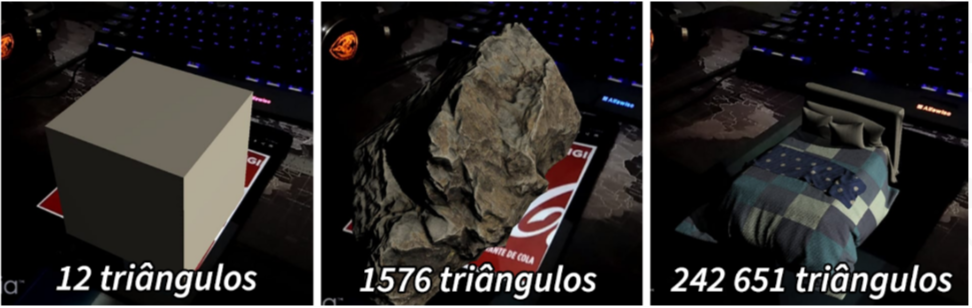
\includegraphics[width=.85\linewidth]{figuras/Vuforia.png}
    \caption{Testes com diferentes modelos de diferentes complexidades, constatando performance acima de 15 quadros por segundo em todos os casos. Fonte: Autor.}
    \label{fig:vuforia-tests}
\end{figure}

As formas de detecção tridimensionais não eram compatíveis com a detecção da posição da cabeça de um paciente, por isso esse recurso não foi testado. O \textit{Vuforia} é uma ferramenta que trabalha com \textit{Android} de \textit{API} 23 ou superior, infelizmente, também incompatível com o \textit{Moverio BT-350} que possui uma \textit{API} 22 e sem chances de atualização. Outras ferramentas foram encontradas como o \textit{Wikitude\texttrademark} que também era para \textit{API} 23 \cite{wikitudes}, porém uma outra ferramenta denominada \textit{ARFoundation} que estima a posição da face humana chamou a atenção por termos a oportunidade de criar uma demonstração da ideia final do projeto nos óculos \cite{arfoundation-docs}.

\begin{figure}[ht]
    \centering
    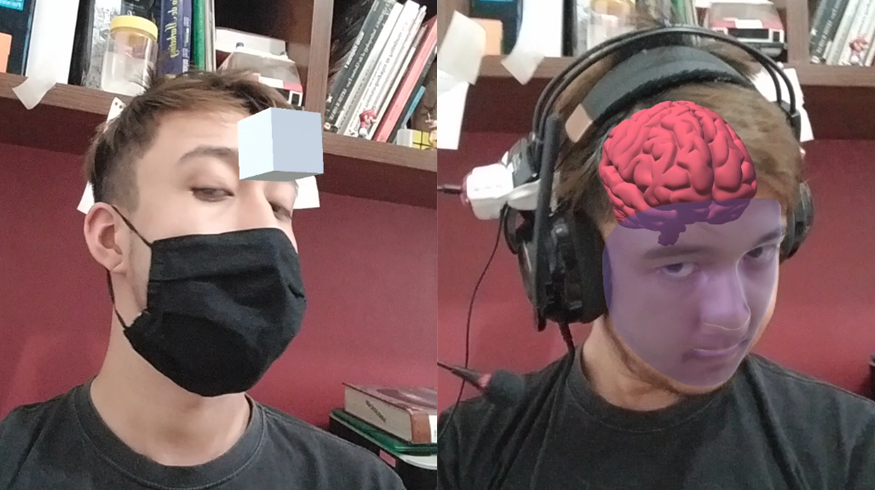
\includegraphics[width=.6\linewidth]{figuras/VCranium.png}
    \caption{A primeira imagem foi o primeiro teste com a projeção de um cubo na região da testa. A segunda detalha a superfície estimada da face e a projeção do cérebro. Fonte: Autor.}
    \label{fig:arfoundation}
\end{figure}

A instalação do \textit{ARFoundation} foi feita no \textit{Unity 2018} e apresentou compatibilidade com celulares de \textit{API 28} ou superior. Os testes consistiram em utilizar a posição da face encontrada pelo \textit{plugin} para projetar um objeto em referência desses dados. A aplicação teve um ótimo resultado e foi possível apresentar o objetivo principal para professores e médicos da área pela aproximação visual dos testes com o resultado final esperado, visto na figura \ref{fig:arfoundation}. Nesse momento, criamos um nome fantasia para facilitar as apresentações do projeto: \textit{VCranium}.

Retornando ao objetivo prático de encontrar um meio de desenvolver o projeto, concluímos que temos muitas opções disponíveis de desenvolvimento, mas sem muito suporte para o \textit{Moverio BT-350}. O \textit{Unity} foi escolhido para seguir a pesquisa pela sua facilidade de elaboração de cenários tridimensionais e compatibilidade com o sistema de outros óculos de AR do mercado. Dessa maneira, podemos garantir que os próximos trabalhos que serão desenvolvidos, não dependem do equipamento que temos hoje, i.e, se futuramente precisarmos trocar para um óculos mais moderno, uma adaptação será feita e aproveitaremos o material produzido até o momento.

Dado o histórico de testes do projeto, foi decidido prosseguir sem depender de \textit{plugins} e bibliotecas \textit{closed-source}, isso garantirá um maior controle do \textit{software} elaborado e também exigirá um estudo mais aprofundado de como os algoritmos de visão computacional funcionam. Essa mudança trará um contato maior com problemas discretizados de programação, auxiliando o processo do estudo e apresentação de dúvidas em seminário para os estudantes e professores dessa área de pesquisa na universidade.

\section{Revisão bibliográfica}

Aqui podemos analisar com mais atenção os artigos da literatura e suas diferentes soluções para sistemas de realidade aumentada aplicados em cirurgias. O trabalho que mais auxiliou a pesquisa foi uma revisão literária de aplicações em AR para neurocirurgias: \textit{"Enhancing Reality: A Systematic Review of Augmented Reality in Neuronavigation and Education"} \cite{enhancedvision}. Esse artigo faz uma breve apresentação da aplicabilidade de AR em ambiente cirúrgico e tabela as informações de doze pesquisas mostrando as patologias tratadas; descrição de método; e resultado da precisão da projeção em AR.

Dentre as pesquisas descritas estava o artigo de Maruyama: \textit{Smart Glasses for Neurosurgical Navigation by Augmented Reality} \cite{Maruyama2018}. Sua equipe de pesquisadores construíram um sistema que utilizava os óculos \textit{Moverio BT-200}, um modelo que se assemelha muito com o que possuímos no laboratório, para auxiliar a visualização de tumores cerebrais em dois pacientes, além disso, foi também possível exibir a escalpe; o crânio; e os vasos da superfície do cérebro nos óculos.

\begin{figure}[ht]
    \centering
    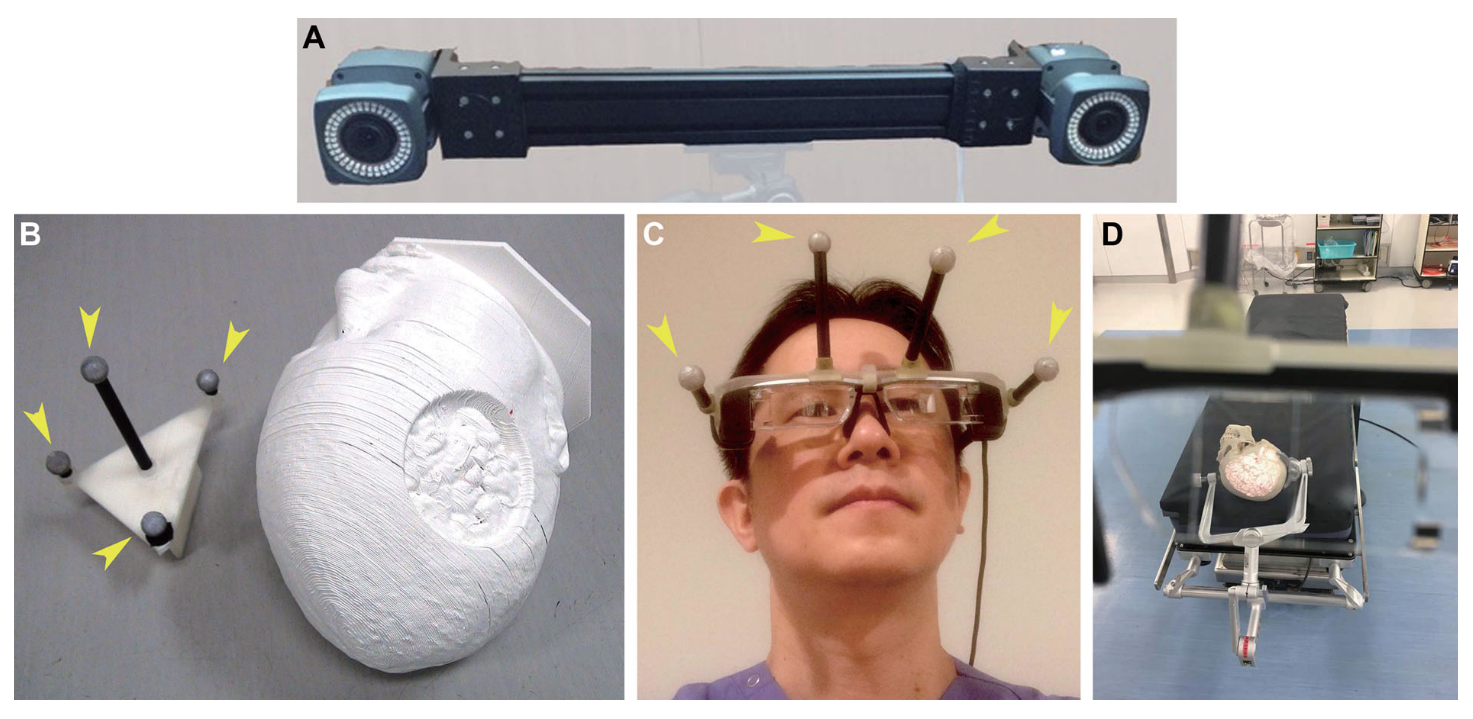
\includegraphics[width=.65\linewidth]{figuras/Maruyama.png}
    \caption{(A) Duas câmeras para detectar movimento, (B) Marcadores para paciente, (C) Marcadores nos óculos, (D) Visualização nos óculos. Fonte: \cite{Maruyama2018}.}
    \label{fig:maruyama}
\end{figure}

O método que o artigo utilizou apresentou a dinâmica da integração de componentes para uma arquitetura de um sistema AR: Empregar câmeras estereoscópicas para a detecção de marcadores nos óculos e na cabeça do paciente; relacionar com os dados da reconstrução 3D do cérebro; utilizar parâmetros da calibração; e fazer a exibição nos óculos. Por meio desse sistema, o resultado obtido é visto na figura \ref{fig:maruyama-overlay}.

\begin{figure}
    \centering
    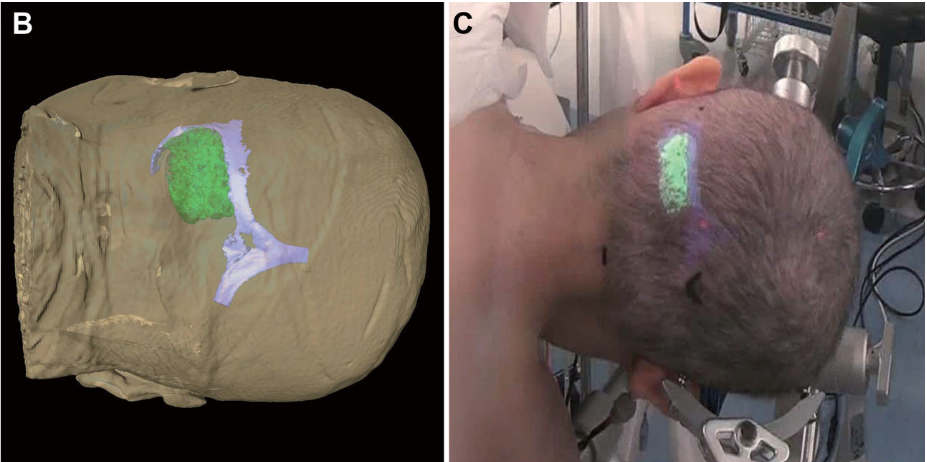
\includegraphics[width=.65\linewidth]{figuras/maruyama-overlay.png}
    \caption{(B) Computação gráfica da reconstrução do cérebro do paciente, (C) Visualização em AR antes da incisão. Fonte: \cite{Maruyama2018}.}
    \label{fig:maruyama-overlay}
\end{figure}

A precisão da projeção, segundo o artigo, foi de \(2.1 \pm  1.3\,mm\) com a mediana de \(1.8\) e a remoção total de \(5\) tumores com sucesso e sem complicações pós-operatórias. Além disso, o sistema tem uma interface de fácil utilização e conveniência para o médico, sendo possível desabilitar a projeção em qualquer momento da cirurgia, teve um custo menor que os sistemas de neuronavegação convencionais e, por fim, pode ser instalado em outros óculos de AR comerciais disponíveis, portanto, não se limitando ao seu modelo do \textit{Moverio} \cite{Maruyama2018}.

Visto os resultados apresentados por essa pesquisa e que a conjectura apresentada na seção anterior - aplicação baseado no \textit{Unity} para a compatibilidade com mais óculos do mercado - foram confirmados possíveis. Contudo, antes de simplesmente seguir os passos de Maruyama, decidimos fazer uma listagem das arquiteturas utilizadas em outros sistemas e tentar ponderar suas características para optarmos pela opção que mais atende as necessidades da pesquisa.

\section{Elaboração do VCranium}

\subsection{Arquitetura do Sistema}

Para a definição de uma arquitetura adequada para o projeto foram analisados os exemplos que a literatura pôde nos dar como

[Fazer Tabela de arquiteturas]

Para esse fim, a equipe realizou reuniões e debates para estabelecer uma solução que seja compatível para um período de seis meses e respeitando as medidas de prevenção por afastamento imposto pela pandemia de COVID-19. Decide-se criar sistema que envolve um computador executando um servidor em \textit{Python}; uma 

% que possui ampla compatibilidade com ferramentas atuais de realidade aumentada, e conectar com os óculos executando uma aplicação \textit{Unity} que posicionaria os objetos 3D na visão do usuário sob as instruções do servidor.

Foram estudados diversos tipos de arquitetura do sistema de projeção em realidade aumentada

A escolha da arquitetura do sistema foi baseada na aplicação dos conceitos menos complexos da visão computacional: a detecção da posição de um marcador no espaço. Essa aplicação foi o ponto de partida de estudos das projeções em realidade aumentada em imagens capturadas por uma câmera.

\begin{figure}[ht]
    \centering
    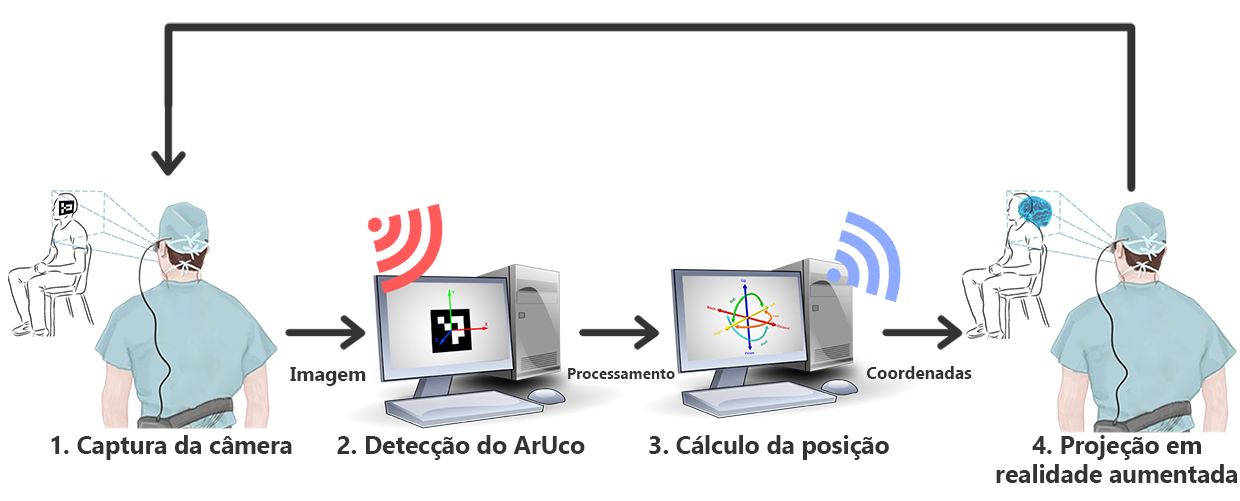
\includegraphics[width=.9\linewidth]{figuras/System schematic.png}
    \caption{A figura representa o funcionamento do sistema. (1) Captura a imagem do paciente e envia para o computador. (2) Faz uma varredura na imagem e identifica o marcador ArUco. (3) Calcula a posição do marcador e envia as coordenadas para os óculos. (4) Recebe as informações e exibe a projeção para o usuário e então retorna para o passo 1. Fonte: Autor.}
    \label{fig:arc}
\end{figure}

% \textbf{Algoritmo de detecção da posição de marcador}
% \textbf{Entrada:} Imagem da câmera
% \textbf{Saída:} Posição do marcador

% \textbf{Etapa 1:} Capture uma imagem da câmera e vá para a Etapa 4, senão há imagem então pare.

% \textbf{Etapa 2:} Identifique o ArUco e vá para a Etapa 3.

% \textbf{Etapa 3:} Estime da posição do marcador no espaço em referência a câmera e retorne à Etapa 1.

% \section{Rascunho}
%% 

% \textit{Vuforia} também tem o suporte do reconhecimento de objetos tridimensionais, porém, os critérios devem ser respeitados:
% \begin{itemize}
%     \item O objeto deve caber no marcador auxiliar (folha A4)
%     \item O objeto não pode conter partes transparentes, translúcidas, luminosas ou reluzentes
%     \item O objeto precisa ter a morfologia (forma) completamente estática
% \end{itemize}

% \begin{figure}[ht]
%     \centering
%     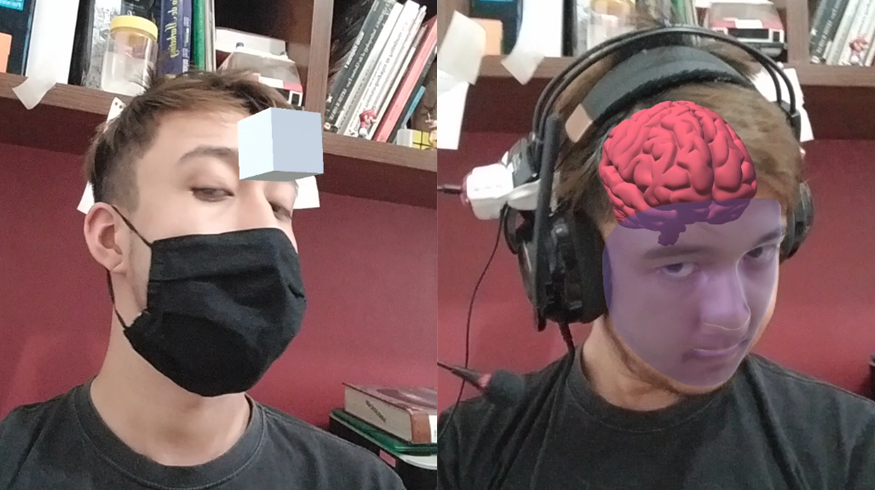
\includegraphics[width=.6\linewidth]{figuras/VCranium.png}
%     \caption{Na esquerda, um teste com um cubo orientado com a face. Na direita, o protótipo do \textit{VCranium} e a exibição do formato de rosto detectado pelo programa. Fonte: Autor.}
%     \label{fig:vcranium}
% \end{figure}

% \begin{figure}[ht]
% \centering
%     \begin{subfigure}{0.45\textwidth}
%         \centering
%         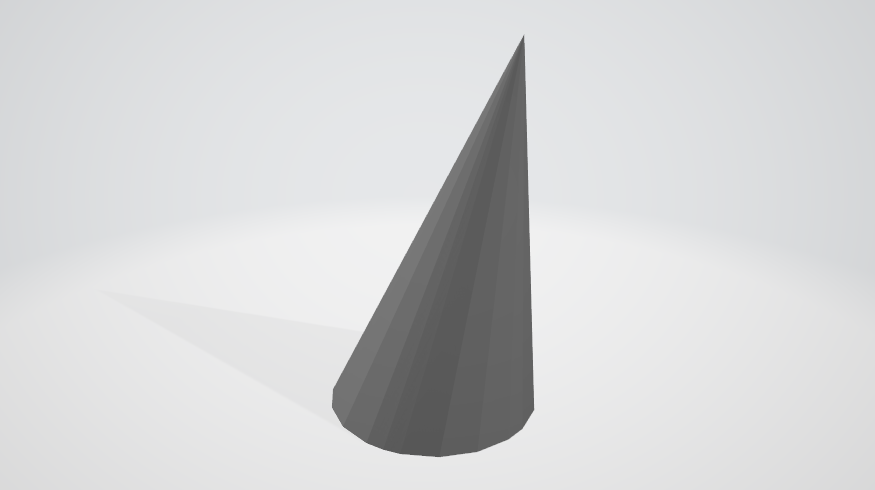
\includegraphics[width=.95\textwidth]{figuras/ConeSTL.png}
%         \caption{Modelo em \textit{STL} do objeto}
%         \label{fig:cone-stl}
%     \end{subfigure}
%     \begin{subfigure}{0.45\textwidth}
%         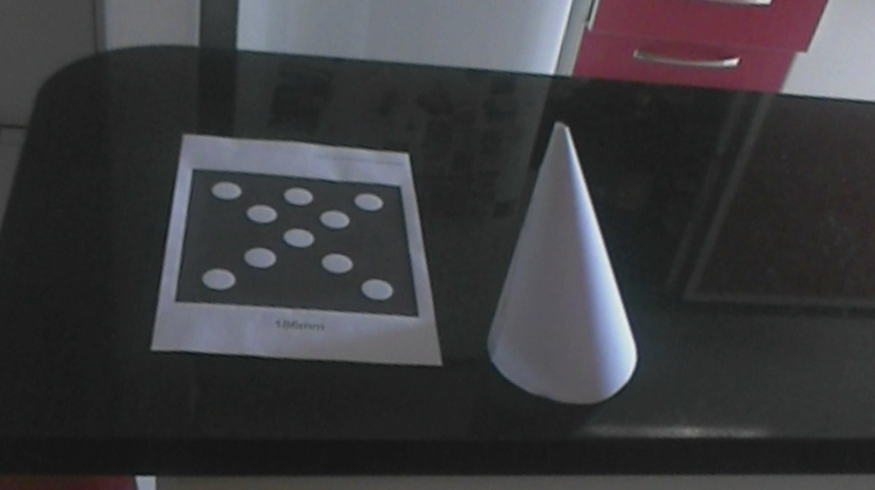
\includegraphics[width=.95\linewidth]{figuras/Cone.png}
%         \caption{Sessão de captura feita em uma mesa preta}
%         \label{fig:cone-training}
%     \end{subfigure}
%     \begin{subfigure}{0.45\textwidth}
%         \centering
%         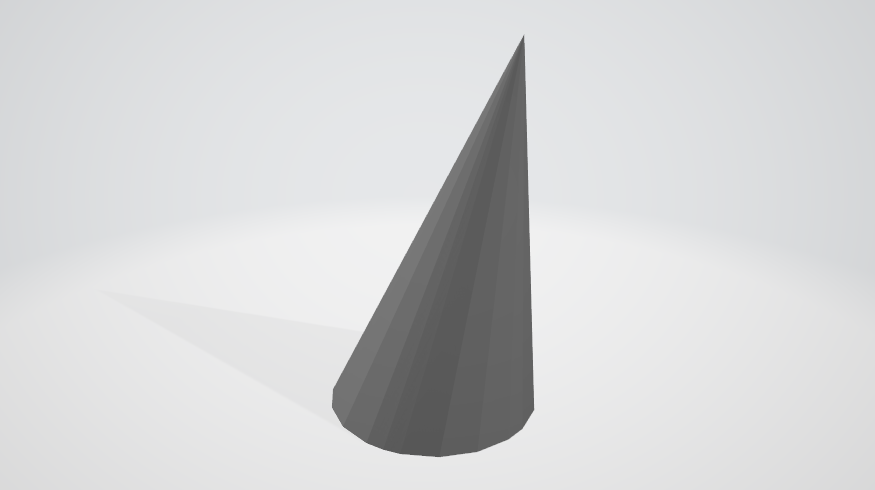
\includegraphics[width=.95\textwidth]{figuras/ConeSTL.png}
%         \caption{Modelo em \textit{STL} do objeto}
%         \label{fig:cone-stl}
%     \end{subfigure}
%     \begin{subfigure}{0.45\textwidth}
%         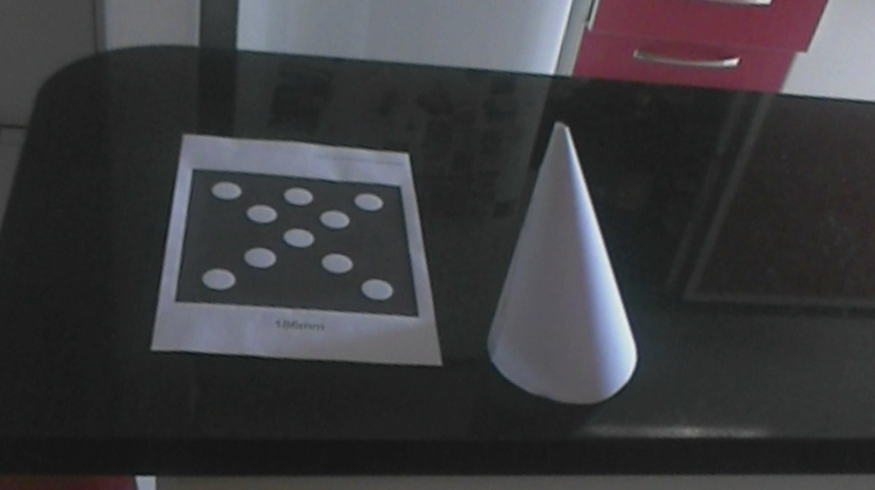
\includegraphics[width=.95\linewidth]{figuras/Cone.png}
%         \caption{Sessão de captura feita em uma mesa preta}
%         \label{fig:cone-training}
%     \end{subfigure}
%     \caption{A tentativa com o cone foi feita em outro ambiente com o fim dar um maior destaque no objeto. Fonte: Autor.}
%     \label{fig:ConeAR}
% \end{figure}

% \begin{center}
% \begin{tabular}{ |c|c| } 
% \hline
% \textbf{Arquivo} & \textit{\textbf{Descrição}} \\ 
% \hline
% \textit{CalibrationTool.apk} & Aplicativo de calibração da projeção da tela dos óculos\\ 
% \hline
% \multirow{2}{*}{\textit{CaptureTool.apk}} & Ferramenta que ajuda a capturar fotos para \\  & o mapeamento de novos marcadores e objetos \\
% \hline
% \multirow{2}{*}{\textit{TrainingToolWindows}} & Usa as imagens obtidas do \textit{CaptureTool.apk} e cria o \\ & \textit{dataset} para a detecção do novo marcador ou objeto  \\
% \hline
% \textit{Moverio\_AR} & Exemplo de cena que aplica funções do \textit{Moverio} no \textit{Unity} \\ 
% \hline
% \end{tabular}
% \end{center}


